\section{Introduction}
\label{intro}
The management of solid waste is one of the most pressing environmental and public-health challenges of the modern era. According to the World Bank, the world generated roughly 2.01 billion tonnes of municipal solid waste in 2016, a figure projected to rise to about 3.40 billion tonnes by 2050 as populations grow and consumption intensifies \cite{whatawaste}. A large and increasing share of this stream is mixed, contaminated, and hazardous, while the sorting infrastructure that must process it, particularly in rapidly urbanizing countries such as Bangladesh, still relies heavily on manual labour. Correct sorting at the point of disposal determines whether a material is recovered for reuse or recycling, sent to landfill, or routed for special hazardous handling; errors are costly both economically, through contaminated and therefore worthless recycling streams, and in terms of safety, when a battery, a medical sharp, or a chemical container is handled as ordinary trash.

Manual sorting is slow, expensive, and, most seriously, dangerous. Workers are routinely exposed to sharp objects, leaking chemicals, and lithium-ion batteries that can ignite, and the cognitive load of distinguishing dozens of material and hazard categories by eye leads to inevitable errors. These pressures motivate automation, and computer vision is the natural enabling technology: a camera observing a disposal point or conveyor can, in principle, recognize what an item is, judge its physical condition, and decide where it should go, far faster and more consistently than a human, and without placing a person in harm's way.

However, most existing vision systems for waste address only a fragment of this problem. They reduce the task to material classification on clean, well-lit, studio-style photographs, and they stop at a coarse ``recyclable versus non-recyclable'' label. Two dimensions that matter enormously for a deployable system are typically missing. The first is the real-world condition of the item: deployment images contain soiling, breakage, deformation, occlusion, background clutter, and uneven lighting that curated benchmarks do not, and an item's condition (for example, intact versus broken glass) can itself change the correct disposal route. The second, and more critical, is the threat an item poses to the people and machinery that must handle it, information that is essential for safe routing but is absent from material-only systems.


\begin{figure}[h]
    \centering
    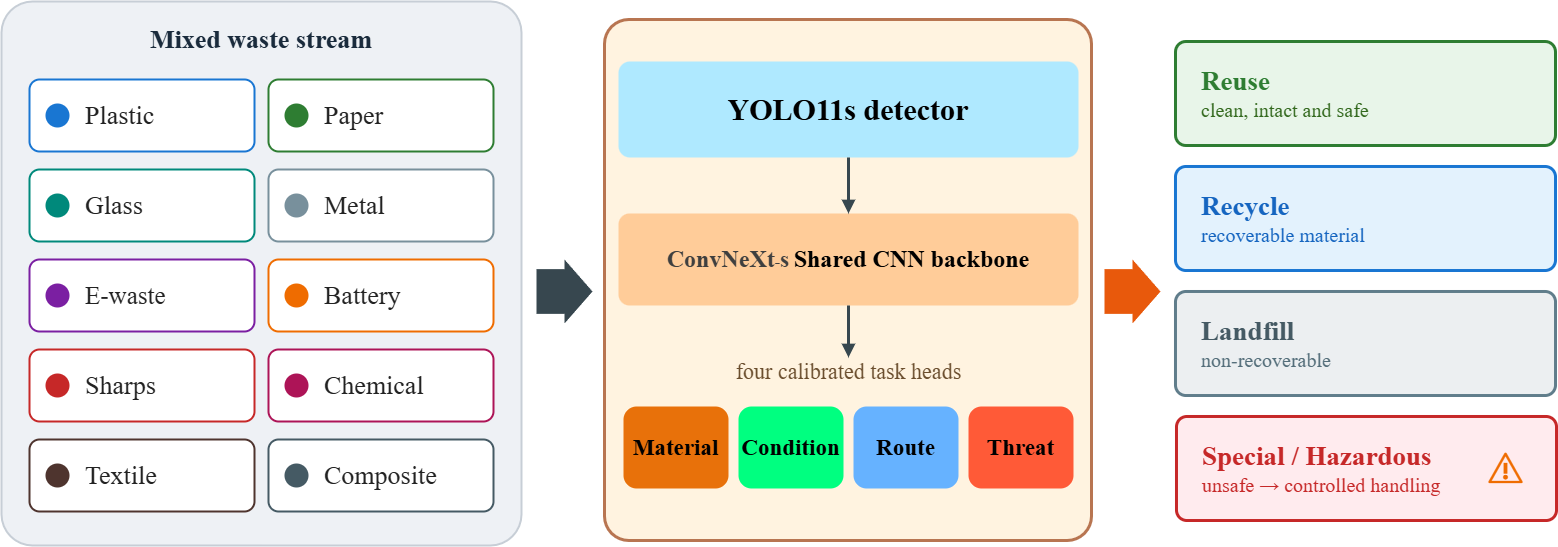
\includegraphics[width=1\textwidth]{./figures/intro_overview.png}
    \caption{High-level overview of the proposed threat-aware, two-stage waste detection and classification system.}
    \label{fig:Overview}
\end{figure}


This thesis addresses both gaps directly; Figure~\ref{fig:Overview} gives a high-level overview of the resulting system. We propose a threat-aware, two-stage detection-and-classification system that operates on real-world-condition images. The system first detects and crops the waste item, then, from a single shared representation, jointly predicts its material across ten classes, its condition, its disposal route, and an ordinal threat level on a four-point severity scale. These four predictions are reconciled by a decision layer grounded in published waste-management regulation and equipped with an explicit safety backstop, so that an item judged to be highly hazardous is routed for special handling even when its material label is visually ambiguous. The result is a complete pipeline (detection, multi-task classification, calibration analysis, and a safety-aware decision) rather than an isolated classifier, and it is evaluated through classification, localization, and routing performance under challenging capture conditions.

\section{Difficulties}
Several challenges were encountered during this research:
\begin{itemize}
    \item \textbf{Real-world image variability:} Unlike curated datasets, the images used here contain genuine variation in lighting, background clutter, occlusion, viewing angle, and physical wear. A robust system must generalize across all of these rather than memorizing clean exemplars.

    \item \textbf{Visual ambiguity of safety-critical classes:} Some of the most important classes are intrinsically hard to separate from appearance alone. A chemical container can look identical to an ordinary plastic or glass bottle, and a composite (multi-material) item visually resembles whichever component is most prominent. These ambiguities make appearance-only classification particularly difficult for the rarest classes.

    \item \textbf{Severe class imbalance and limited data:} The taxonomy includes both common streams (e.g., plastic) and scarce but critical ones (e.g., hazardous chemical, composite), with only a few dozen items in the smallest classes. Training and, especially, evaluating such rare classes reliably is difficult.

    \item \textbf{Modelling threat as an ordered quantity:} Threat severity is not a set of unrelated categories but an ordered scale; a model should be penalized more for confusing ``low'' with ``high'' than ``low'' with ``moderate.'' This requires an ordinal formulation rather than ordinary classification.

    \item \textbf{Computational constraints:} Training nine deep backbones, six object detectors, and a cross-validation study under a fixed GPU budget required careful, efficient experimental design.
\end{itemize}

\section{Applications}
\begin{itemize}
    \item \textbf{Automated and assisted sorting:} The system is intended to support a sorting station (on a conveyor, at a collection point, or as a phone/edge application) by recognizing the item and recommending a disposal route.

    \item \textbf{Worker and public safety:} By explicitly predicting threat level and directing predicted hazardous items to special handling, the system targets the most dangerous and most under-studied part of waste sorting: sharps, batteries, electronic waste, and chemicals.

    \item \textbf{Recycling-stream quality:} Correct material and condition prediction can reduce contamination of recyclable streams, improving the value and recoverability of collected material.

    \item \textbf{Decision support and auditing:} Because the decision layer is rule-based and produces an explanation and a confidence value for each item, its outputs can be audited and deferred to a human when uncertain.

    \item \textbf{Regulatory alignment:} Routing is grounded in published waste-management regulations, so the system's recommendations map to actual local disposal streams rather than abstract labels.
\end{itemize}

\section{Motivation}
The motivation for this research arises from the following considerations:
\begin{itemize}
    \item \textbf{Safety first:} Mis-handling hazardous waste endangers sanitation workers and the public. A system that treats threat as a first-class output and provides a prediction-based safety backstop directly addresses a problem that material-only classifiers ignore.

    \item \textbf{Realism over benchmarks:} Studio-condition accuracy does not necessarily transfer to deployment. Training and evaluating under genuine real-world condition is necessary for the results to be meaningful.

    \item \textbf{Trustworthy automation:} For automation to be adopted, its confidences must be reliable and it must be able to abstain. Calibration analysis and a confidence-aware decision layer address these requirements.

    \item \textbf{Local relevance:} Grounding the routing rules in Bangladesh's solid-waste regulations and the national 3R strategy makes the system relevant to the context in which it would be deployed.
\end{itemize}

\section{Contribution of the thesis}
This thesis makes the following contributions:
\begin{itemize}
    \item It formulates waste handling as a four-head multi-task problem (material, condition, route, and an ordinal threat level) on a shared backbone, rather than as isolated material classification. To our knowledge, modelling disposal-threat severity as a rank-consistent ordinal head wired into a decision cost is novel in the waste computer-vision literature.

    \item It implements a complete two-stage detect-then-classify pipeline (YOLO11s detector followed by the multi-task classifier) and shows no measurable drop in material accuracy versus an oracle crop on 50 test items (accuracy 0.840 for both, at a detection rate of 1.0), although condition and route scores decrease slightly.

    \item It introduces a regulation-grounded decision layer with confidence-aware reconciliation and abstention, and a threat-based safety backstop that directs predicted hazardous items to special handling regardless of their predicted material. Per-head temperature calibration is evaluated to assess confidence quality.

    \item It provides a rigorous evaluation: a comparison of ten classifier configurations spanning convolutional and transformer backbones and an ensemble, cross-validated evaluation over 457 items with bootstrap 95\% confidence intervals, calibration analysis, paired significance testing, external validation on public datasets, and an honest, evidence-based analysis of the hardest rare classes.
\end{itemize}

\section{Thesis Organization}
The remainder of this report is organized as follows:
\begin{itemize}
    \item \textbf{Chapter 2} reviews related work on waste detection and classification, threat/hazard handling, ordinal regression, and calibration, and identifies the gaps this thesis addresses.
    \item \textbf{Chapter 3} describes the proposed methodology, from dataset construction and the labelling scheme through the detector, the multi-task network, the loss functions, the training recipe, and the decision layer.
    \item \textbf{Chapter 4} presents the experimental results and analysis, including the backbone ablation, the cross-validated headline results, detection and external validation, and the rare-class analysis.
    \item \textbf{Chapter 5} concludes the thesis, summarizing the findings and outlining limitations and directions for future work.
\end{itemize}

\section{Conclusion}
This chapter introduced the problem of threat-aware waste detection and classification under real-world condition, motivated the need to model both item condition and handling threat alongside material and route, and summarized the difficulties, applications, and contributions of the work. The following chapter situates the proposed system within the existing literature.
